\documentclass{article}
\usepackage{amsfonts, amsthm, amsmath, amssymb, mathtools, ulem, mathrsfs, physics, esint, siunitx, tikz-cd}
\usepackage{pdfpages, fullpage, color, microtype, cancel, textcomp, markdown, hyperref, graphicx}
\usepackage{enumitem}
\usepackage{algorithm}
\usepackage{algpseudocode}
\graphicspath{{./images/}}
\usepackage[english]{babel}
\usepackage[autostyle, english=american]{csquotes}
\MakeOuterQuote{"}
\usepackage{xparse}
\usepackage{tikz}

\usepackage{calligra}
\DeclareMathAlphabet{\mathcalligra}{T1}{calligra}{m}{n}
\DeclareFontShape{T1}{calligra}{m}{n}{<->s*[2.2]callig15}{}
\newcommand{\script}[1]{\ensuremath{\mathcalligra{#1}}}
\newcommand{\scr}{\script r}

% fonts
\def\mbb#1{\mathbb{#1}}
\def\mfk#1{\mathfrak{#1}}
\def\mbf#1{\mathbf{#1}}
\def\tbf#1{\textbf{#1}}

% common bold letters
\def\bP{\mbb{P}}
\def\bC{\mbb{C}}
\def\bH{\mbb{H}}
\def\bI{\mbb{I}}
\def\bR{\mbb{R}}
\def\bQ{\mbb{Q}}
\def\bZ{\mbb{Z}}
\def\bN{\mbb{N}}

% brackets
\newcommand{\br}[1]{\left(#1\right)}
\newcommand{\sbr}[1]{\left[#1\right]}
\newcommand{\brc}[1]{\left\{#1\right\}}
\newcommand{\lbr}[1]{\left\langle#1\right\rangle}

% vectors
\renewcommand{\i}{\hat{\imath}}
\renewcommand{\j}{\hat{\jmath}}
\renewcommand{\k}{\hat{k}}
\newcommand{\proj}[2]{\text{proj}_{#2}\br{#1}}
\newcommand{\m}[2][b]{\begin{#1matrix}#2\end{#1matrix}}
\newcommand{\arr}[3][\sbr]{#1{\begin{array}{#2}#3\end{array}}}

% misc
\NewDocumentCommand{\seq}{O{n} O{1} O{\infty} m}{\br{#4}_{{#1}={#2}}^{#3}}
\NewDocumentCommand{\app}{O{x} O{\infty}}{\xrightarrow{#1\to#2}}
\newcommand{\sm}{\setminus}
\newcommand{\sse}{\subseteq}
\renewcommand{\ss}{\subset}
\newcommand{\vn}{\varnothing}
\newcommand{\lc}{\epsilon_{ijk}}
\newcommand{\ep}{\epsilon}
\newcommand{\vp}{\varphi}
\renewcommand{\th}{\theta}
\newcommand{\cjg}[1]{\overline{#1}}
\newcommand{\inv}{^{-1}}
\DeclareMathOperator{\im}{im}
\DeclareMathOperator{\id}{id}
\newcommand{\imp}{\implies}
\newcommand{\impleft}{\reflectbox{$\implies$}}
\newcommand{\ck}{\frac1{4\pi\ep_0}}
\newcommand{\ckb}{4\pi\ep_0}
\newcommand{\sto}{\longrightarrow}
\DeclareMathOperator{\cl}{cl}
\DeclareMathOperator{\intt}{int}
\DeclareMathOperator{\bd}{bd}
\DeclareMathOperator{\Span}{span}
\newcommand{\floor}[1]{\left\lfloor#1\right\rfloor}
\newcommand{\ceil}[1]{\left\lceil#1\right\rceil}
\newcommand{\fxn}[5]{#1:\begin{array}{rcl}#2&\longrightarrow & #3\\[-0.5mm]#4&\longmapsto &#5\end{array}}
\newcommand{\sep}[1][.5cm]{\vspace{#1}}
\DeclareMathOperator{\card}{card}
\renewcommand{\ip}[2]{\lbr{#1,#2}}
\renewcommand{\bar}{\overline}
\DeclareMathOperator{\cis}{cis}
\DeclareMathOperator{\Arg}{Arg}
\newcommand{\ptl}{\partial}

% title
\title{Scientific Computing HW 8}
\author{Ryan Chen}
%\date{\today}
\setlength{\parindent}{0pt}


\begin{document}
	
\maketitle



\begin{enumerate}
	


\item

\begin{enumerate}
	
	
	\item The matrix $G$ is given by
	$$G = A\inv \m{0 & 0 \\ 1 & 0 \\ 0 & 1},
	\quad A := \m{1 & 1 & 1 \\ x_1 & x_2 & x_3 \\ y_1 & y_2 & y_3}$$
	We find $A\inv$ by its adjugate. By cofactor expansion over the first row,
	$$D := \det(A)
	= \m[v]{x_2 & x_3 \\ y_2 & y_3} - \m[v]{x_1 & x_3 \\ y_1 & y_3} + \m[v]{x_1 & x_2 \\ y_1 & y_2}
	= x_2y_3 - x_3y_2 - x_1y_3 + x_3y_1 + x_1y_2 - x_2y_1$$
	The matrix of cofactors is
	$$\mathrm{cof}(A) = \m{x_2y_3-x_3y_2 & -x_1y_3+x_3y_1 & x_1y_2-x_2y_1 \\ -y_3+y_2 & y_3-y_1 & -y_2+y_1 \\ x_3-x_2 & -x_3+x_1 & x_2-x_1}$$
	The adjugate of $A$ is
	$$\mathrm{adj}(A) = \mathrm{cof}(A)^T
	= \m{x_2y_3-x_3y_2 & -y_3+y_2  & x_3-x_2 \\ -x_1y_3+x_3y_1& y_3-y_1 & -x_3+x_1 \\ x_1y_2-x_2y_1 & -y_2+y_1 & x_2-x_1}$$
	Thus
	$$G = \frac{1}{D}\mathrm{adj}(A)\m{0 & 0 \\ 1 & 0 \\ 0 & 1}
	= \frac{1}{D}\m{y_2-y_3 & x_3-x_2 \\ y_3-y_1 & x_1-x_3 \\ y_1-y_2 & x_2-x_1}$$
	
	Fix an even permutation $(i,j,k)$ of $1,2,3$ (i.e. one of $(1,2,3),~(2,3,1),~(3,1,2)$).
	$$\eta_i(x,y) = \frac{\m[v]{1 & x & y \\ 1 & x_j & y_j \\ 1 & x_k & y_k}}{\m[v]{1 & x_i & y_i \\ 1 & x_j & y_j \\ 1 & x_k & y_k}}$$
	Since the permutation $(i,j,k)$ is even, the denominator is $\det(A^T)=\det(A)=D$. By cofactor expansion over the first row, the numerator is $x_jy_k - x_ky_j - (y_k - y_j)x + (x_k - x_j)y$, so that
	$$\ptl_x\eta_i(x,y) = \frac{1}{D}(y_j-y_k),
	\quad \ptl_y\eta_i(x,y) = \frac{1}{D}(x_k-x_j)$$
	Thus
	$$\m{\ptl_x\eta_1(x,y) & \ptl_y\eta_1(x,y) \\ \ptl_x\eta_2(x,y) & \ptl_y\eta_2(x,y) \\ \ptl_x\eta_3(x,y) & \ptl_y\eta_3(x,y)}
	= \frac{1}{D}\m{y_2-y_3 & x_3-x_2 \\ y_3-y_1 & x_1-x_3 \\ y_1-y_2 & x_2-x_1}
	= G$$
	
	
	\item Using the functions $\eta_j$ from (a) and the fact $\grad\eta_j$ is the $j$th row of $G$,
	$$u(x,y) = \sum_{j=1}^3 u_j\eta_j(x,y)
	\imp \grad u(x,y) = \sum_{j=1}^3 u_j \grad\eta_j(x,y)
	= \frac{1}{D}\br{u_1\m{y_2-y_3 \\ x_3-x_2} + u_2\m{y_3-y_1 \\ x_1-x_3} + u_3\m{y_1-y_2 \\ x_2-x_1}}$$
	$$\imp \grad u(x,y) = (x_2y_3 - x_3y_2 - x_1y_3 + x_3y_1 + x_1y_2 - x_2y_1)\inv\m{u_1(y_2-y_3)+u_2(y_3-y_1)+u_3(y_1-y_2) \\ u_1(x_3-x_2)+u_2(x_1-x_3)+u_3(x_2-x_1)}$$
	
	
\end{enumerate}


	
\item 

Code: \url{https://github.com/RokettoJanpu/scientific-computing-2-redux/blob/main/hw8.ipynb}

These functions were written:
\begin{itemize}
	\item a\_func: Determine the conductivity at a point.
	\item find\_vert\_line\_pts: Find the mesh points along a given vertical line
	\item FEM\_hw\_solver: FEM solver for the BVP in the HW.
\end{itemize}

We use the function distmesh2D to generate the mesh. For the fixed points, we pick the corners of the square and 100 evenly spaced points on the circle with center $(1.5,1.5)$ and radius 1.
\begin{center}
	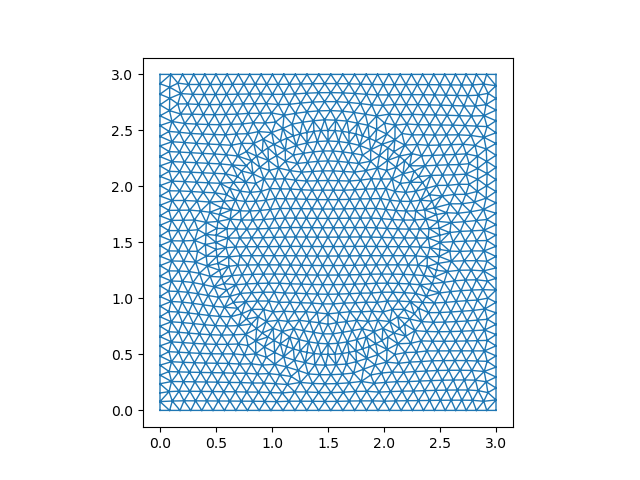
\includegraphics[scale=.5]{hw8 mesh}
\end{center}

We solve for the voltage with the function FEM\_hw\_solver. We then plot the voltage and the current density.
\begin{itemize}
	\item For $a_1=1.2$ and $a_2=1$:
	\begin{center}
		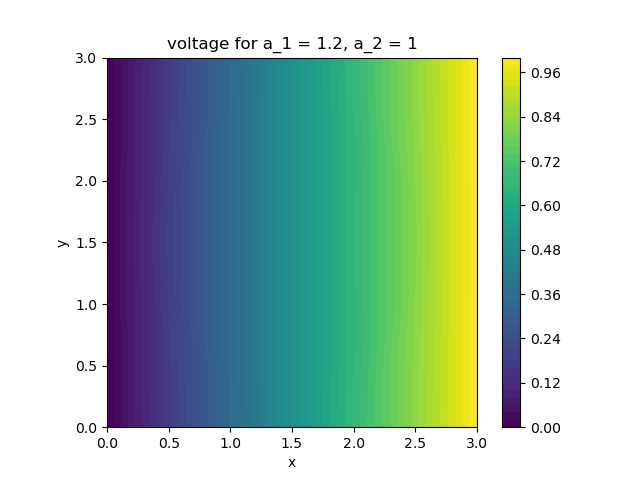
\includegraphics[scale=.4]{hw8 voltage 1}
		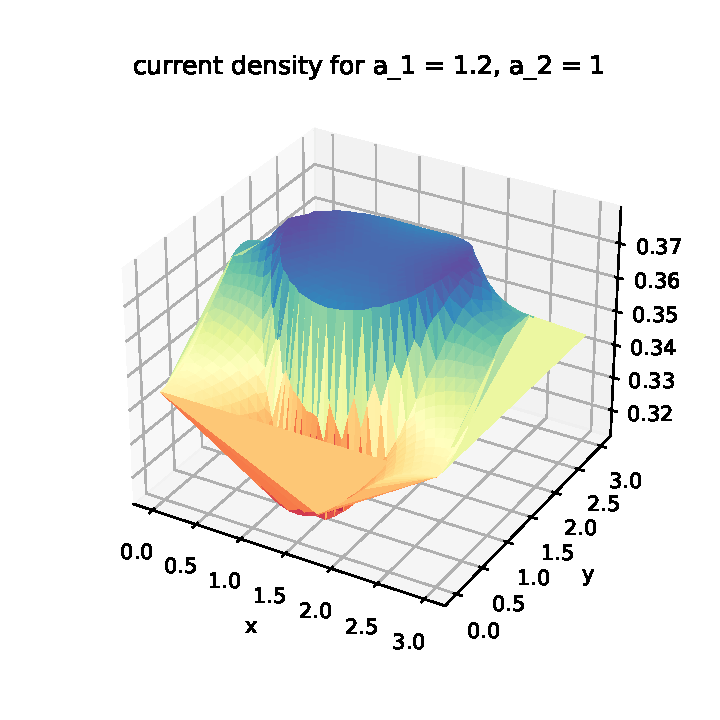
\includegraphics[scale=.4]{hw8 current 1}
	\end{center}
	Note that in this case $a_1>a_2$, which visually corresponds to the fact that the current density is greater on the inside of the circle than the outside.
	\item For $a_1=0.8$ and $a_2=1$:
	\begin{center}
		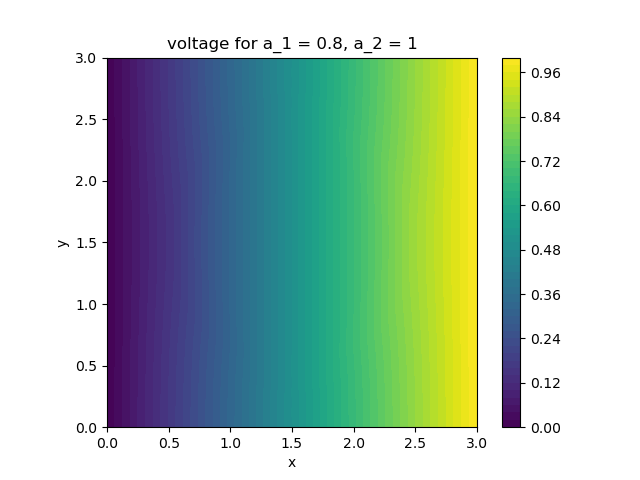
\includegraphics[scale=.4]{hw8 voltage 2}
		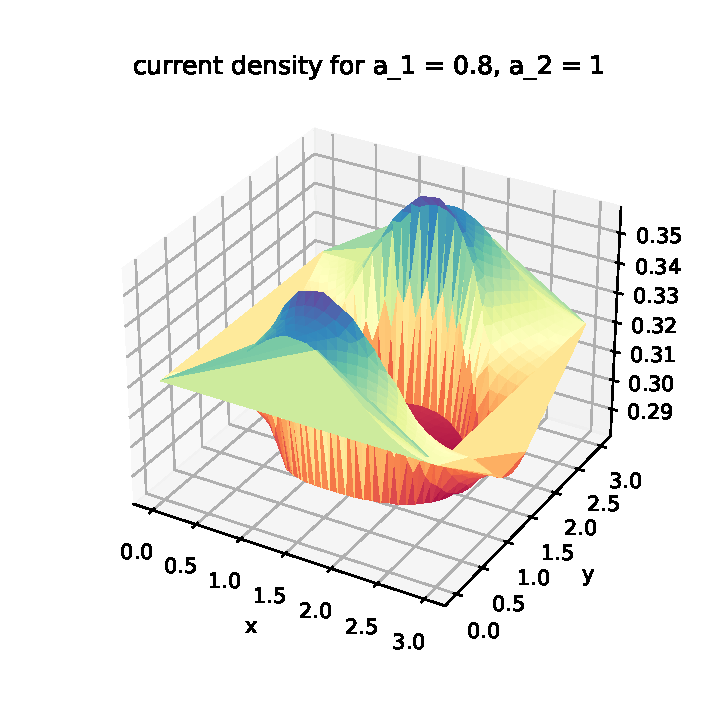
\includegraphics[scale=.4]{hw8 current 2}
	\end{center}
	Note that in this case $a_1<a_2$, which visually corresponds to the fact that the current density is greater on the outside of the circle than the inside.
\end{itemize}
These cases illustrate the principle of ``the path of least resistance'', in the sense that current flow is higher in regions of greater electrical conductivity.



\item

\begin{enumerate}
	
	
	\item Write
	$$u(x) = \int_0^1 G(x,y)f(y)dy
	= \int_0^x G(x,y)f(y)dy + \int_x^1 G(x,y)f(y)dy$$
	$$= (1-x)\int_0^x yf(y)dy + x\int_x^1 (1-y)f(y)dy
	= (1-x)\int_0^x yf(y)dy - x\int_1^x (1-y)f(y)dy$$
	Then compute
	$$u'(x) = -\int_0^x yf(y)dy + (1-x)xf(x) - \int_1^x (1-y)f(y)dy - x(1-x)f(x)$$
	$$= -\int_0^x yf(y)dy - \int_1^x f(y)dy + \int_1^x yf(y)dy
	= -\int_1^x f(y)dy$$
	$$\imp u''(x) = -f(x)$$
	
	
	\item Compute
	$$\ptl_yG(x,y) =
	\begin{cases}
		1-x, & y<x\\
		-x, & y>x
	\end{cases}$$
	Then
	$$\int_0^1 v'(y)\ptl_yG(x,y)dy = \int_0^x v'(y)\ptl_yG(x,y)dy + \int_x^1 v'(y)\ptl_yG(x,y)dy$$
	$$= (1-x)\int_0^x v'(y)dy - x\int_x^1 v'(y)dy
	= \int_0^x v'(y)dy - x\int_0^x v'(y)dy - x\int_x^1 v'(y)dy
	= \int_0^x v'(y)dy - x\int_0^1 v'(y)dy$$
	$$= v(x) - v(0) - x[v(1) - v(0)]
	= v(x) - 0 - x[0 - 0]
	= v(x)$$
	Since $u\in H^1_0([0,1])$, the identity in particular holds for $u$.
	
	
	\item The linear interpolant $I_hu$, as a linear combination of the basis functions $\phi_j$, is
	$$I_hu = \sum_{j=1}^n u(x_j)\phi_j$$
	
	
	\item The function
	$$\psi_j(x) := G(x_j,y) =
	\begin{cases}
		(1-x_j)y, & y\le x_j\\
		x_j(1-y), & y>x_j
	\end{cases}$$
	satisfies $\psi_j(0)=\psi_j(1)=0$ and is linear on each interval $[x_i,x_{i+1}]$ for $0\le i\le n$, so $\psi_j\in S_h$. Also note that $\psi_j$ is not differentiable at $x_j$, but is differentiable at all other points.
	
	Suppose the functions $\psi_j$ are linearly dependent, i.e. there exist scalars $c_j$, not all 0, so that
	$$\sum_{j=1}^nc_j\psi_j=0$$
	In particular the linear combination
	$$\sum_{j=1}^nc_j\psi_j$$
	is differentiable. From the assumption we can pick $i$ so that $c_i\ne0$. Since the functions $\psi_j$, for $j\ne i$, are differentiable at $x_i$, the linear combination
	$$\sum_{j=1 \atop j\ne i}^n c_j\psi_j$$
	is differentiable at $x_i$. Also, since $\psi_i$ is not differentiable at $x_i$ and $c_i\ne0$, the function $c_i\psi_i$ is not differentiable at $x_i$. This means the linear combination $\sum_{j=1}^nc_j\psi_j$ is not differentiable at $x_i$, a contradiction. Thus the functions $\psi_j$ are linearly independent.
	
	Lastly, since $\dim(S_h)=n$, the $n$ linearly independent functions $\psi_j$ form a basis of $S_h$.
	
	
	\item Recall that
	$$\ptl_yG(x,y) =
	\begin{cases}
		1-x, & y<x\\
		-x, & y>x
	\end{cases},
	\quad \phi_i'(x) =
	\begin{cases}
		0, & x<x_{i-1} \text{ or } x>x_{i+1}\\
		\frac{1}{x_i-x_{i-1}}, & x_{i-1}<x<x_i\\
		-\frac{1}{x_{i+1}-x_i}, & x_i<x<x_{i+1}
	\end{cases}$$
	First write
	$$\int_0^1 [I_hu]'(y)\ptl_yG(x_j,y)dy
	= \int_0^1 \sbr{\sum_{i=1}^n u(x_i)\phi_i'(y)}\ptl_yG(x_j,y)dy$$
	$$= \sum_{i=1}^n u(x_i)\int_0^1 \phi_i'(y)\ptl_yG(x_j,y)dy
	= \sum_{i=1}^n u(x_i)\underbrace{\int_{x_{i-1}}^{x_{i+1}} \phi_i'(y)\ptl_yG(x_j,y)dy}_{=:a_{ij}}$$
	
	Now examine cases.
	\begin{itemize}
		
		\item If $i=j$,
		$$a_{ij} = \int_{x_{j-1}}^{x_j}\frac{1-x_j}{x_j-x_{j-1}}dy + \int_{x_j}^{x_{j+1}}\frac{-x_j}{-(x_{j+1}-x_j)}dy
		= 1 - x_j + x_j
		= 1$$
		
		\item If $i\ge j+1$,
		$$a_{ij} = \int_{x_{i-1}}^{x_i}\frac{-x_j}{x_i-x_{i-1}}dy + \int_{x_i}^{x_{i+1}}\frac{-x_j}{-(x_{i+1}-x_i)}dy
		= -x_j + x_j
		= 0$$
		
		\item If $i\le j-1$,
		$$a_{ij} = \int_{x_{i-1}}^{x_i}\frac{1-x_j}{x_i-x_{i-1}}dy + \int_{x_i}^{x_{i+1}}\frac{1-x_j}{-(x_{i+1}-x_i)}dy
		= 1 - x_j - (1 - x_j)
		= 0$$	
		
	\end{itemize}
	This means $a_{ij}=\delta_{ij}$, thus
	$$\int_0^1 [I_hu]'(y)\ptl_yG(x_j,y)dy = \sum_{i=1}^n u(x_i)\delta_{ij} = u(x_j)$$

\end{enumerate}



\item

\begin{enumerate}
	
	\item Using the identity $\div(fv)=\grad f\cdot v+f\div v$ for any scalar function $f$ and vector field $v$,
	$$\div(e^{-\beta V(x)}\grad u) + \beta e^{-\beta V(x)}f(x)\cdot\grad u
	= e^{-\beta V(x)}\Delta u - \beta e^{-\beta V(x)}\grad V(x)\cdot\grad u + \beta e^{-\beta V(x)}f(x)\cdot\grad u$$
	$$= \beta e^{-\beta V(x)}\sbr{\beta\inv\Delta u - \grad V(x)\cdot\grad u + f(x)\cdot\grad u}
	= \beta e^{-\beta V(x)}\sbr{\beta\inv\Delta u + b(x)\cdot\grad u}$$
	and since $\beta e^{-\beta V(x)}\ne0$ for all $x$,
	$$\beta\inv\Delta u + b(x)\cdot\grad u = 0
	\iff \div(e^{-\beta V(x)}\grad u) + \beta e^{-\beta V(x)}f(x)\cdot\grad u = 0$$
	hence the two BVPs are equivalent.
	
	
	\item Decompose
	$$b(x,y) = \m{x-x^3-10xy^2 \\ -y-x^2y}
	= \underbrace{\m{x-x^3-xy^2 \\ -y-3y^3-x^2y}}_{=:F(x,y)} + \underbrace{\m{-9xy^2 \\ 3y^3}}_{=:f(x,y)}$$
	We check
	$$\curl F = \ptl_x(-y-3y^3-x^2y) + \ptl_y(x-x^3-xy^2) = -2xy + 2xy = 0$$
	$$\div f = \ptl_x(-9xy^2) + \ptl_y(3y^3) = -9y^2 + 9y^2 = 0$$
	so the decomposition is as desired. For the vector field
	$$-F(x,y) = \m{-x+x^3+xy^2 \\ y+3y^3+x^2y}$$
	a potential $V$ is found by
	$$V(x,y) = \int (-x+x^3+xy^2)dx = -\frac12x^2 + \frac14x^4 + \frac12x^2y^2 + g(y)$$
	for some function $g$, and
	$$V(x,y) = \int (y+3y^3+x^2y)dy = \frac12y^2 + \frac34y^4 + \frac12x^2y^2 + h(x)$$
	for some function $h$. Putting the calculations together,
	$$V(x,y) = -\frac12x^2 + \frac14x^4 + \frac12x^2y^2 + \frac12y^2 + \frac34y^4$$

 
\end{enumerate}



\end{enumerate}

	
\end{document}